

\textbf{Golang}


Uno de los puntos centrales de este trabajo es exponer el estado del arte en el uso de Golang para el entorno industrial. En dicho estudio se ha consultado distintos papers y publicaciones para extraer primeras conclusiones:

Uno de los puntos más importantes para el desarrollo de software industrial es los recursos consumidos una de las primeras conclusines extraidas de la eficiencia del uso de golang interaccionando con mysql, una de las combinaciones más comerciales concluye que: "... combination of Go and MySQL is superior regarding CPU utilization and memory usage, while Node.js and MySQL combination is superior regarding response time~\cite{Effendy20211955}".

Un estudio más centrado en el uso de recursos ante problemas de algorítmia con altos requerimientos, en particular la implementacion de un árbol de decisiones. ~\cite{Dymora20201} Donde encontramos un punto importante: golang vuelve a no dar ventajas, pero tampoco inconvenientes en materia de tiempos de ejecucion. pero si que pierde en uso de cpu claramente y empata en materia de uso de memoria para mas de 500K registros en este problema en particular. Aunque se admite que la optimización de dicho mecanismo para este problema. lo cual es posible. "Thus, the Go language garbage collector
supports programmers by automatically releasing their programs’ memory when it is no longer needed.
However, tracking and cleaning the memory requires additional resources such as CPU time. The effect
of this can be seen in Figure 5. Of course, the scope of optimizing"~\cite{Dymora20201}

lo que si nos permite extraer es una conclusion y es que para usos intensivos golang es una opción viable pero no da ventaja en este aspecto.

Esto se debe al mecanismo que le da una ventaja tan notoria en el uso menos intensivo: el garbage collector que le requiere un uso adicional de memoria y cpu para ejecuciones con un gran número de registros. Concluye este estudio diciendo: ". Go can be an
attractive alternative in the area of DevOps tools. It is attractive to build something small–medium
that works natively without using a lot of RAM and which runs fast with many things needed for
this task in the language itself"~\cite{Dymora20201}

\begin{figure}[H]
	\centering
	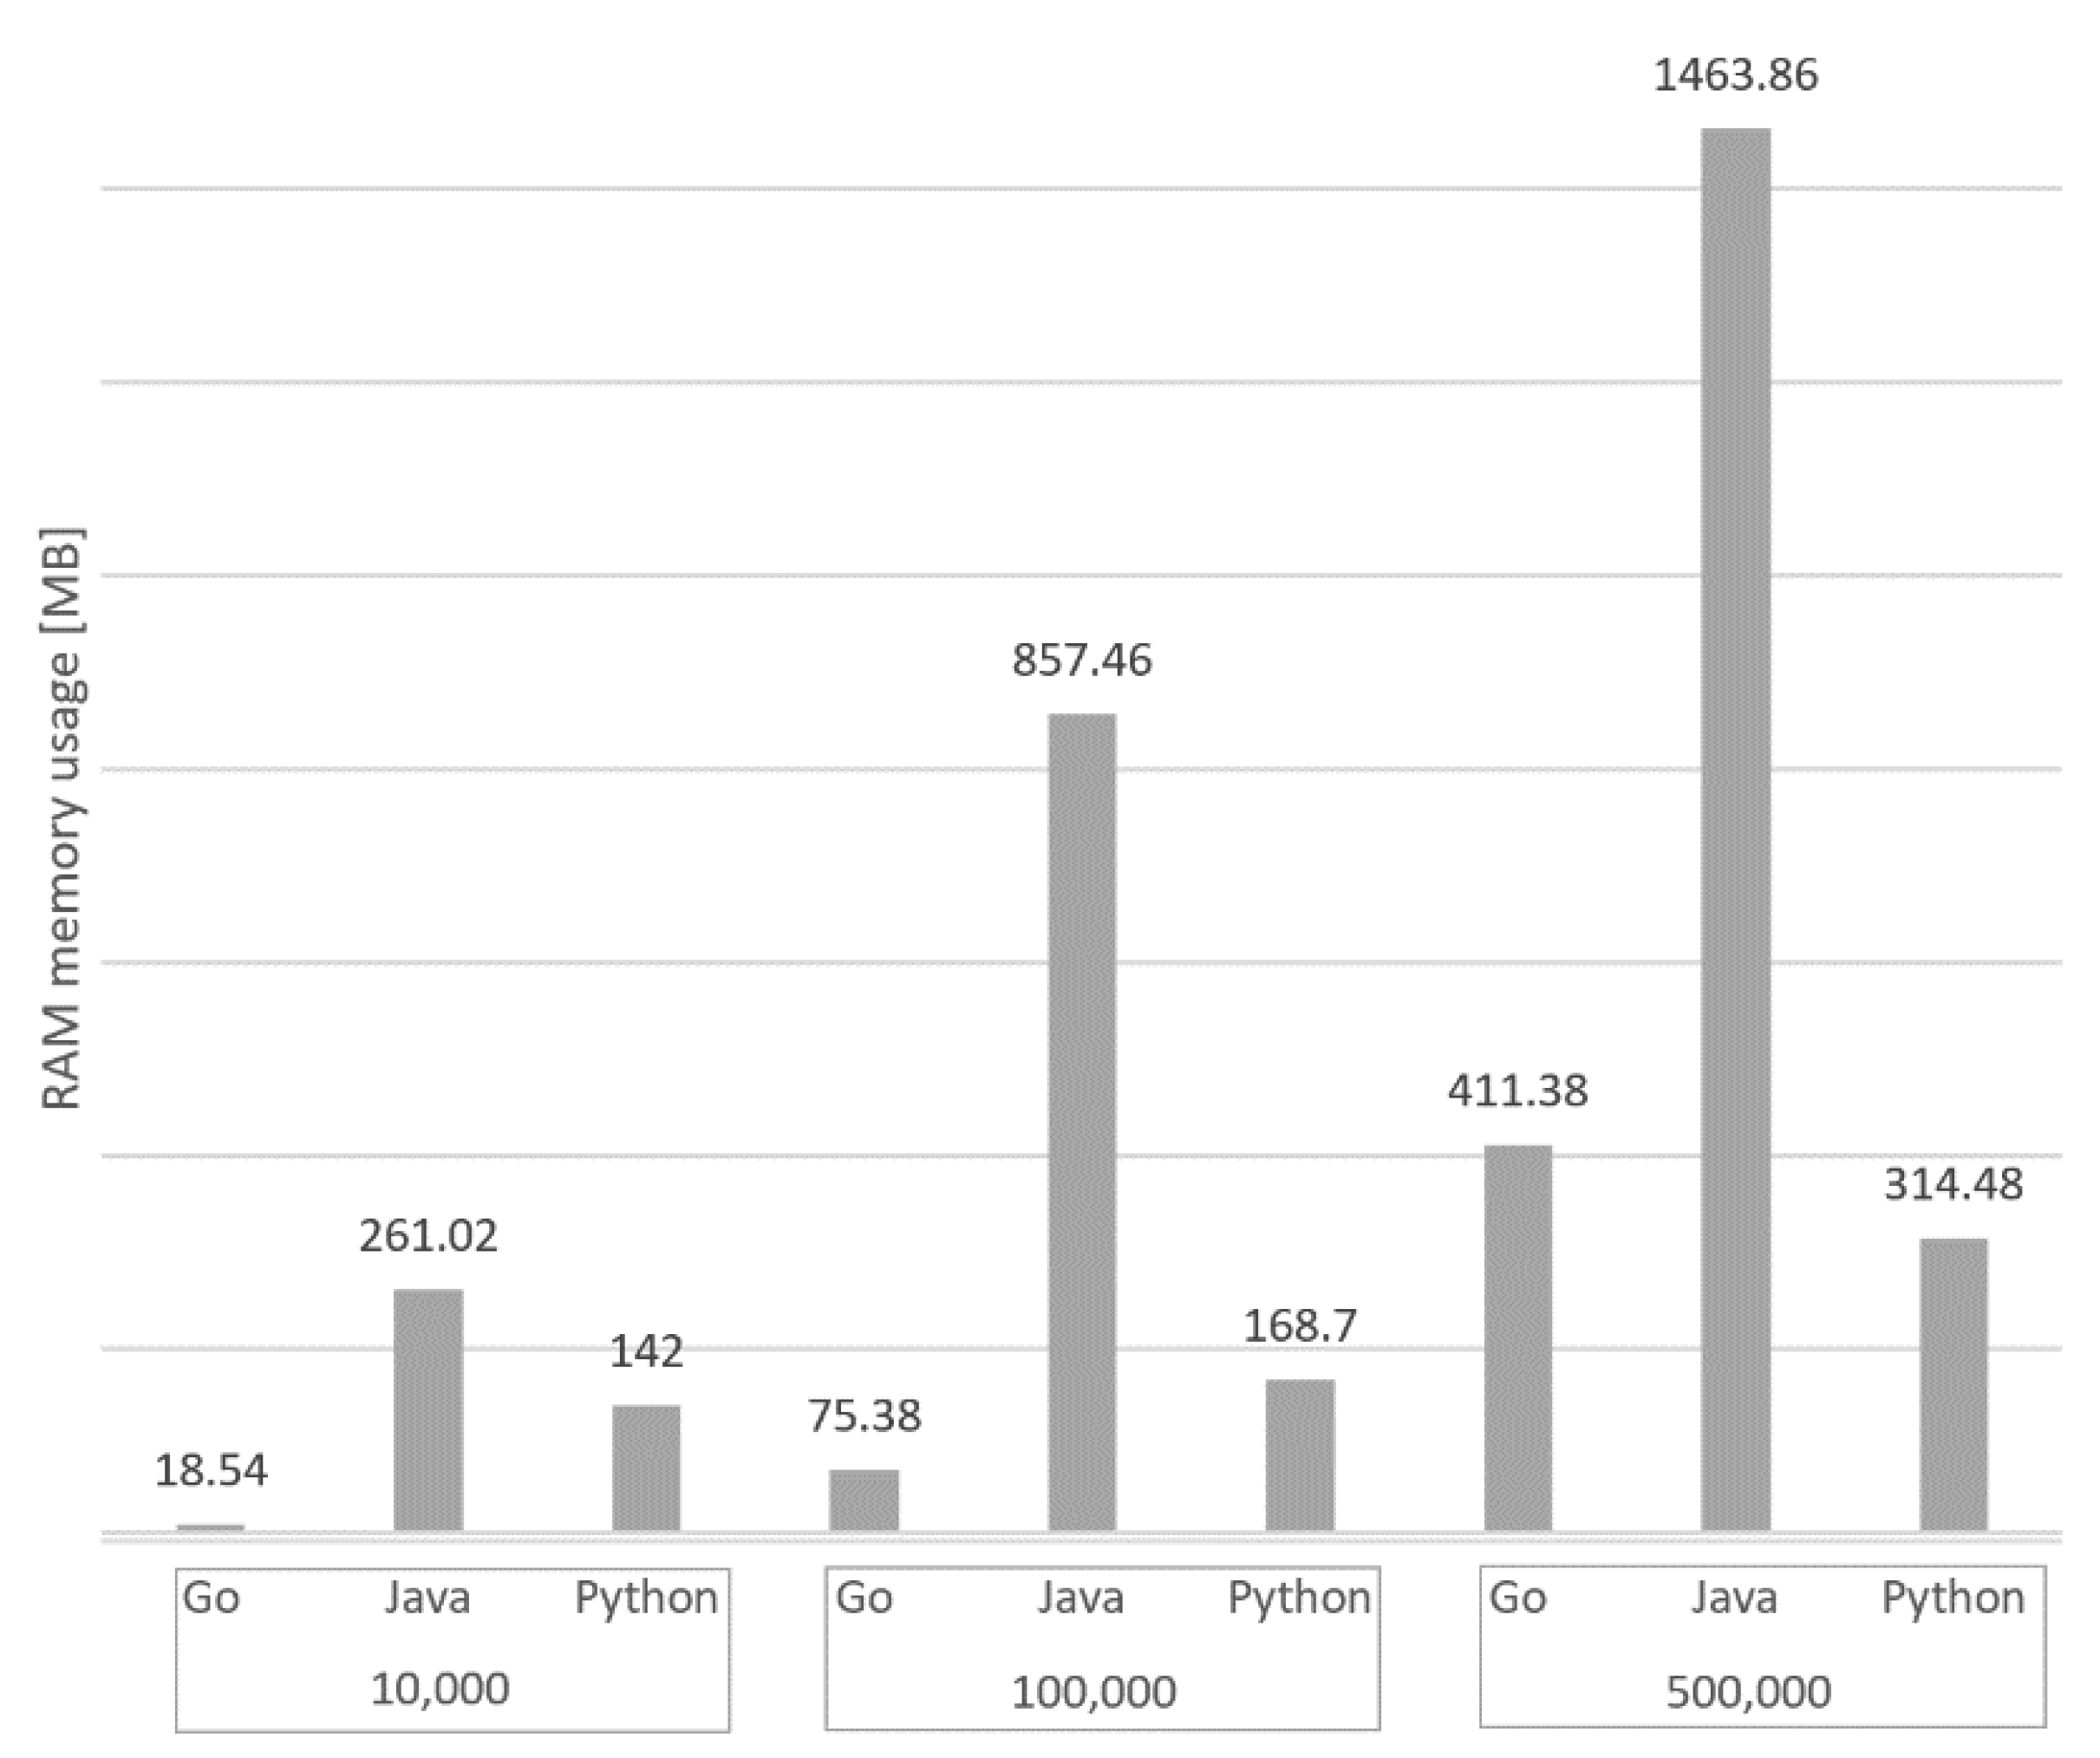
\includegraphics[height=0.3\textheight]{./part/Proyecto_ejecutivo/memoria_constructiva/golang/img/memory_usage}
	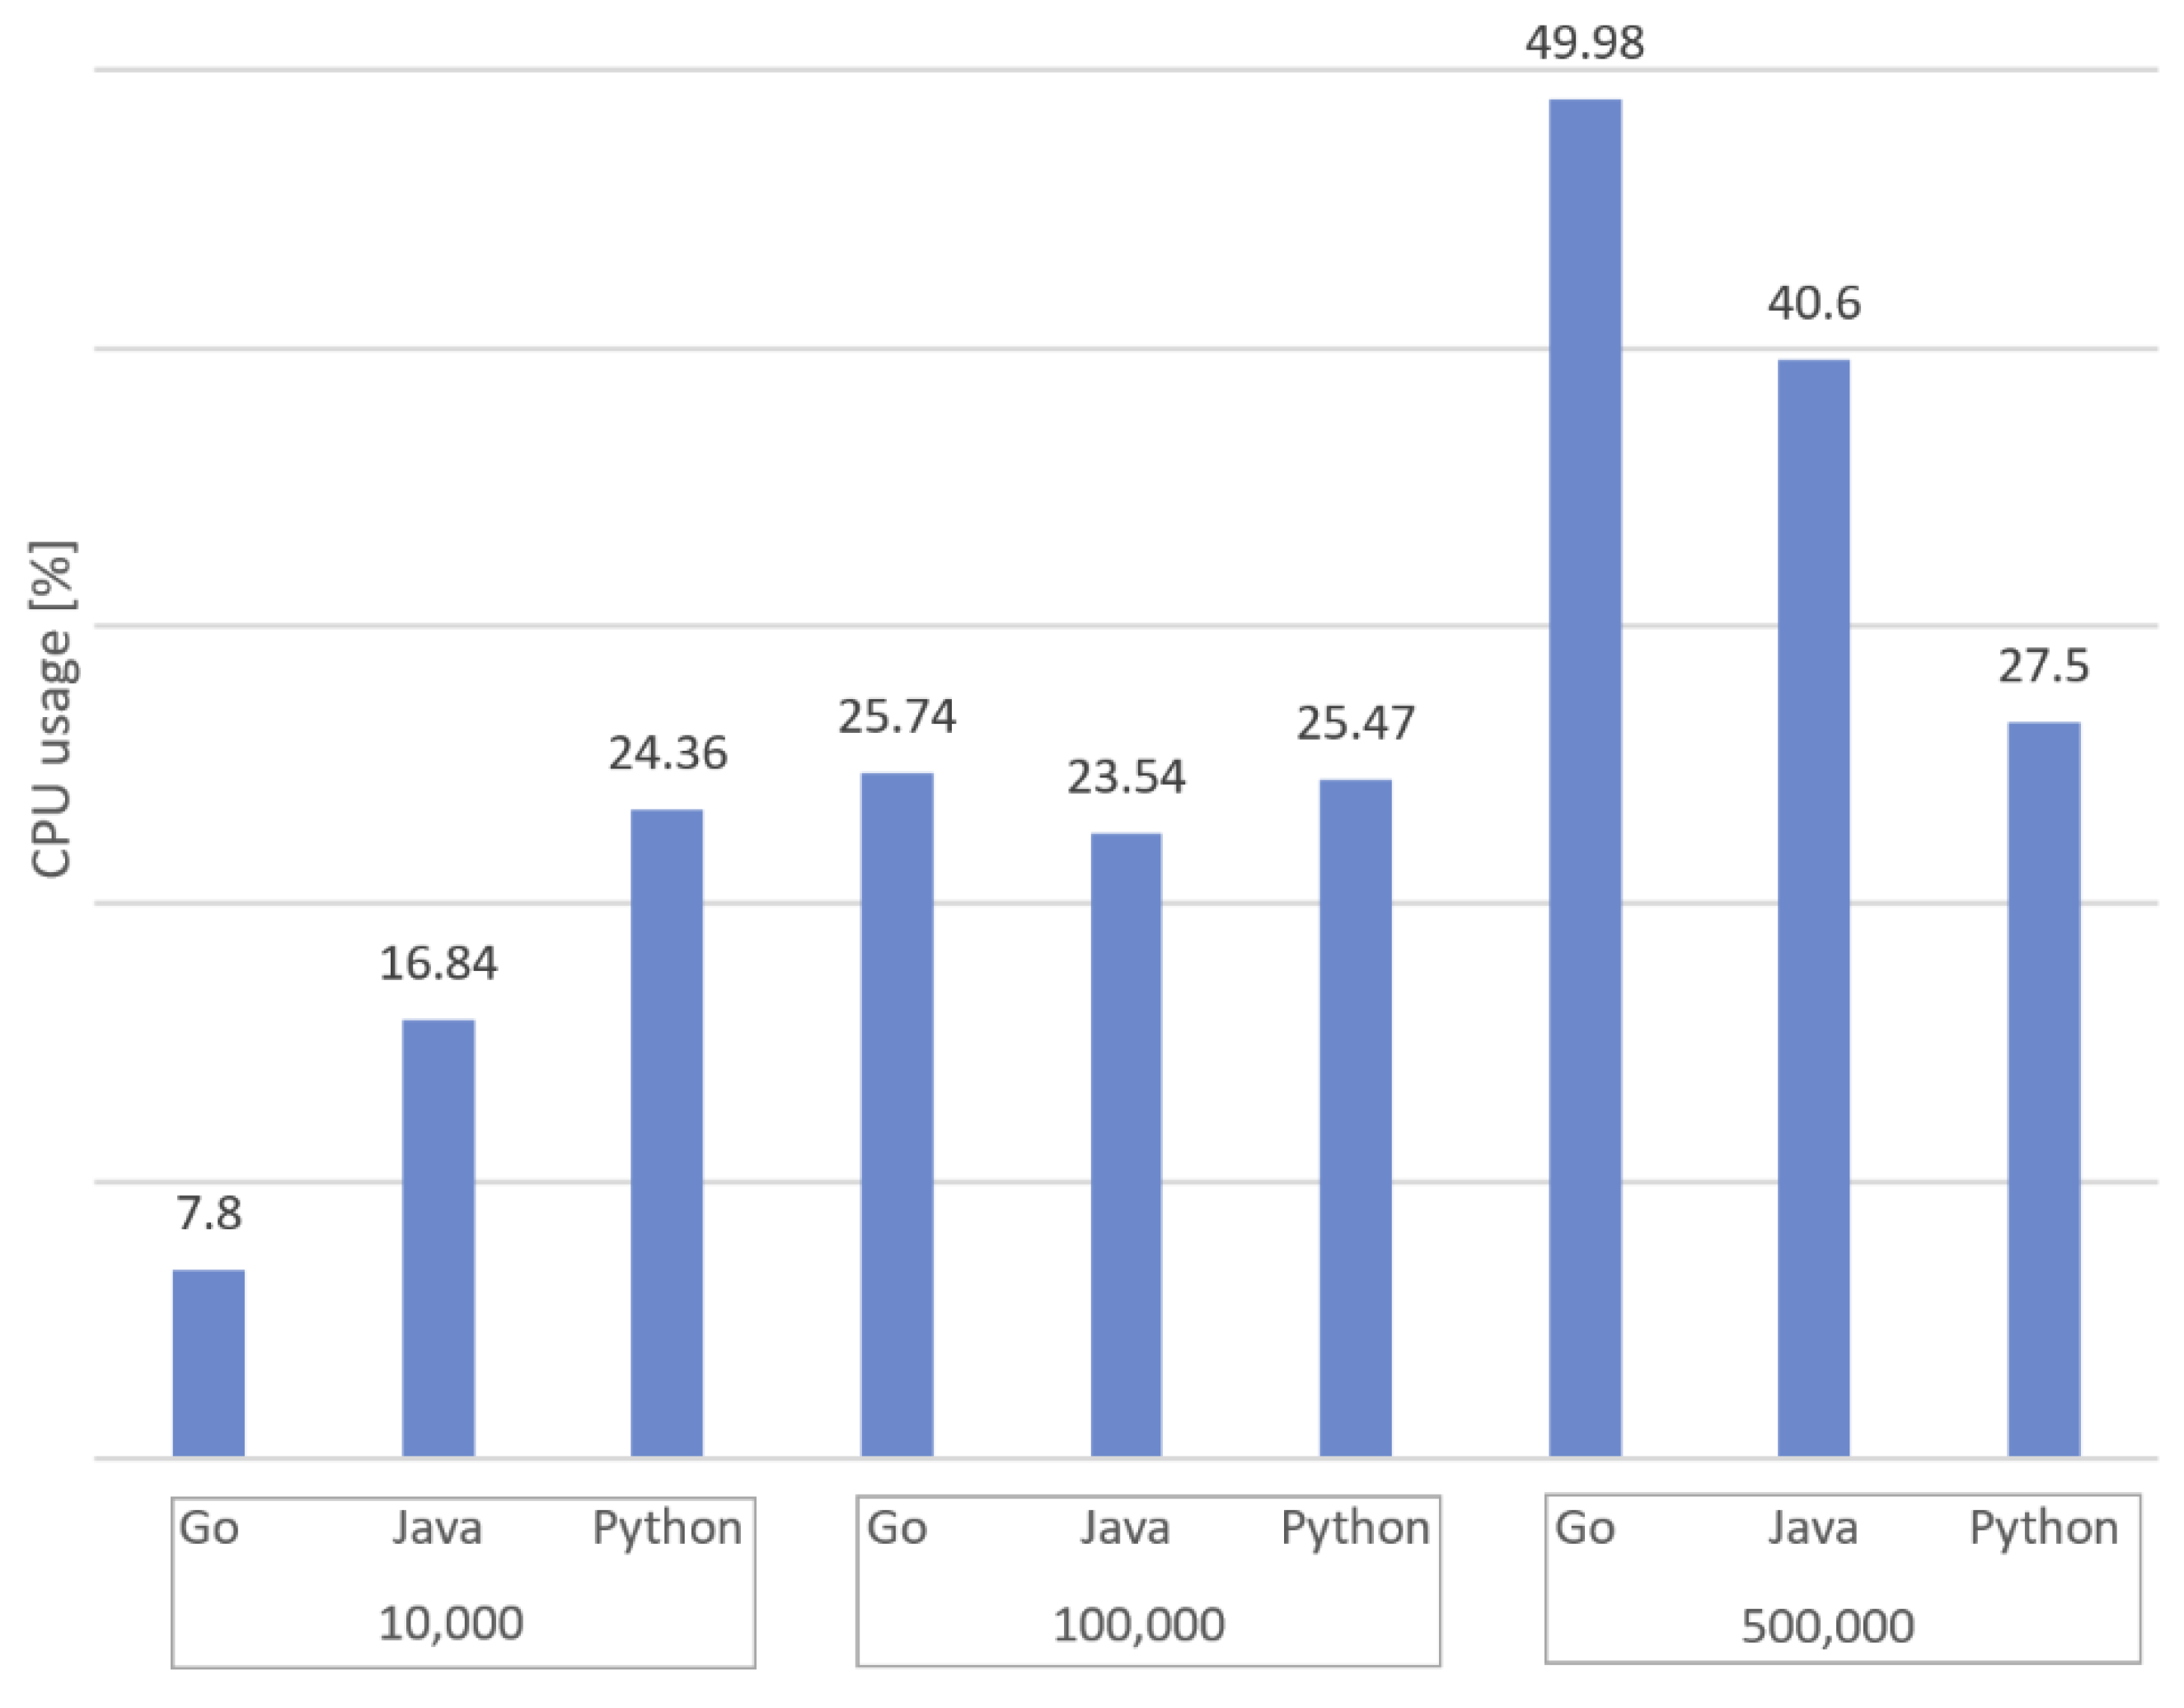
\includegraphics[height=0.3\textheight]{./part/Proyecto_ejecutivo/memoria_constructiva/golang/img/cpuUsage}
	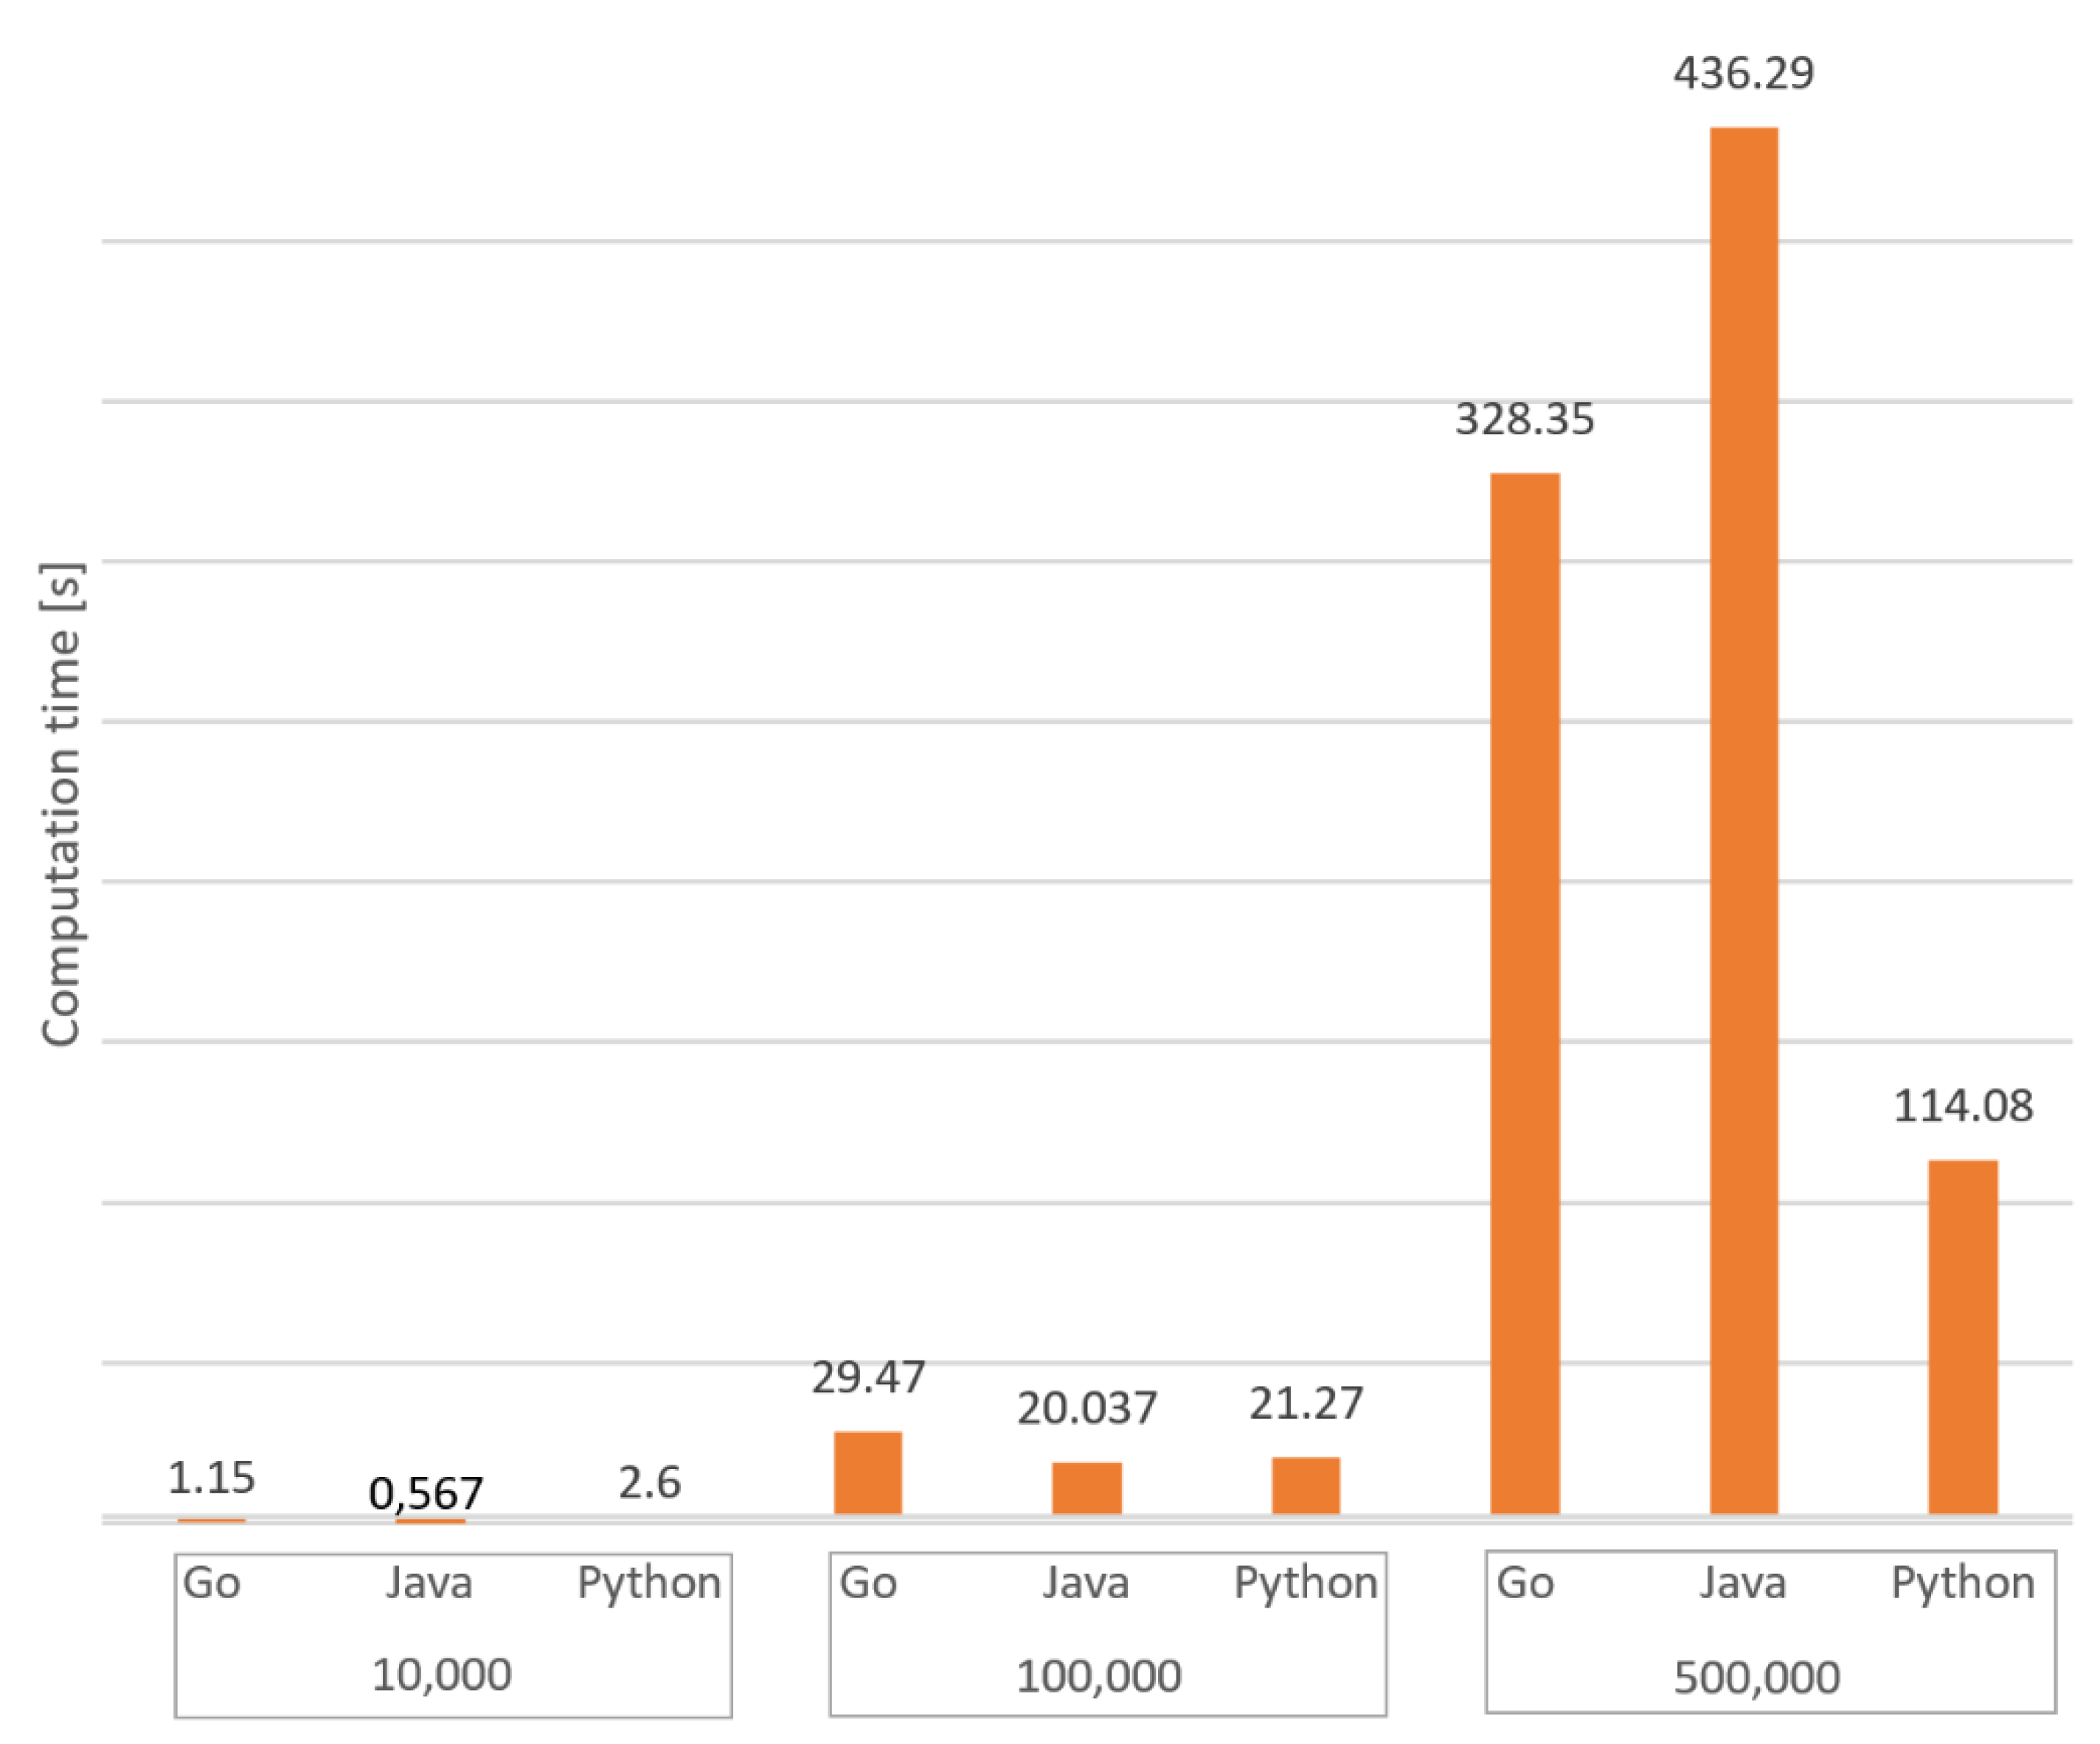
\includegraphics[height=0.3\textheight]{./part/Proyecto_ejecutivo/memoria_constructiva/golang/img/compTime}
	\caption[performance golang on algorithm]{performance golang on algorithm\cite{Dymora20201}}\label{fig:performance golang}
\end{figure}

El verdadero motivo para optar por golang como lenguaje para un software viene más de la mano de la facilidad de mantenimiendo, la rapidez de compilacion, el manejo fácil para la concurrencia y eficiente en el uso de recursos. Implementar mecanismos de memoria compartida para procesos concurrente es donde golang si optimiza recursos. Uno de los trabajadores de google que ha contribuido al ecosistema de go nos dice "Everyone knows and thinks about Google in terms of scale of users and scale of servers, but one thing that's not talked about as often is the scale of engineering effort."~\cite{Meyerson2014104+101}

Esto quiere decir que en la mayoría de las compañías el mayor coste no es el de infraestructura, si no el de ingeniería. Es un tradeoff muy importante el reducir el numero de horas dedicadas a mantener y desarrollar software que el hecho de optimizar el uso de máquinas. Si encima nos encontramos con un problema que no requiere de uso intensivo en cuestión algorítmica o tiempo de respuesta encontramos lo mejor de los dos: tenemos la ventaja de reducir los recuros necesarios de infraestructura y los de ingeniería. Si se diera el caso de que el software se enfrenta con el tiempo a problemas de escala siempre nos quedará la opción de aumentar las prestaciones de las máquinas utilizadas pero no tener problemas de aumento de costes de ingeniería

Es en la implementación de algoritmos que sacan ventaja de la concurrencia donde golang puede sacar ventaja respecto a otros lenguages como java o python ~\cite{Jenkins201714}

Estas son las principales conclusiones extraidas de la lectura de las publicaciones consultadas.
\cite{Effendy20211955}
\cite{Dymora20201}
\cite{Meyerson2014104+101}
\cite{Ray202110857}
\cite{Jenkins201714}
\cite{Ding2021321}
\cite{Taheri2021138}
\cite{NoAuthor2021179}
\cite{Dilley2019377}
\cite{Qiu2018}
\cite{Shoumik20181}
\cite{Mladenovic2018}
\cite{Benedict2017437}
\cite{Irawan2017}
\cite{Samaniego2017116}
\cite{Khaitan20152909}
\cite{Leokhin2015656}
\cite{Komendantskaya2014121}
\cite{Mittal2014292}
\cite{WhiteheadII2011209}
Nos permiten concluir que está justificado el uso en nuestro objetivo de diseñar un sistema de las carácteristicas de este proyecto con Golang.

Concluyo mencionando \cite{WhiteheadII2011209}"Despite the relatively young age of the programming language, we believe that Go helps
to fill an interesting niche in the field of programming languages. The unique feature-set and
aims of the language make it worth investigation for systems-level concurrent programming." Habiendo madurado el lenguaje unos años desde la publicación de este artículo encontramos que sigue siendo interesante, está altamente valorado en la comunidad.

